%%%%%%%%%%%%%%%%%%%%%%%%%%%%%%%%%%%%%%%%%
% Programming/Coding Assignment
% LaTeX Template
%
% This template has been downloaded from:
% http://www.latextemplates.com
%
% Original author:
% Ted Pavlic (http://www.tedpavlic.com)
%
% Note:
% The \lipsum[#] commands throughout this template generate dummy text
% to fill the template out. These commands should all be removed when 
% writing assignment content.
%
% This template uses a Perl script as an example snippet of code, most other
% languages are also usable. Configure them in the "CODE INCLUSION 
% CONFIGURATION" section.
%
%%%%%%%%%%%%%%%%%%%%%%%%%%%%%%%%%%%%%%%%%

%----------------------------------------------------------------------------------------
%	PACKAGES AND OTHER DOCUMENT CONFIGURATIONS
%----------------------------------------------------------------------------------------

\documentclass{article}

\usepackage{fancyhdr} % Required for custom headers
\usepackage{lastpage} % Required to determine the last page for the footer
\usepackage{extramarks} % Required for headers and footers
\usepackage[usenames,dvipsnames]{color} % Required for custom colors
\usepackage{graphicx} % Required to insert images
\usepackage{listings} % Required for insertion of code
\usepackage{courier} % Required for the courier font
\usepackage{tikz}
\usepackage[latin1]{inputenc}
\usetikzlibrary{shapes,arrows}

% Margins
\topmargin=-0.45in
\evensidemargin=0in
\oddsidemargin=0in
\textwidth=6.5in
\textheight=9.0in
\headsep=0.25in

\linespread{1.1} % Line spacing

% Set up the header and footer
\pagestyle{fancy}
\lhead{\hmwkAuthorName} % Top left header
\chead{\hmwkClass\ (\hmwkClassInstructor\ \hmwkClassTime): \hmwkTitle} % Top center head
\rhead{\firstxmark} % Top right header
\lfoot{\lastxmark} % Bottom left footer
\cfoot{} % Bottom center footer
\rfoot{Page\ \thepage\ of\ \protect\pageref{LastPage}} % Bottom right footer
\renewcommand\headrulewidth{0.4pt} % Size of the header rule
\renewcommand\footrulewidth{0.4pt} % Size of the footer rule

\setlength\parindent{0pt} % Removes all indentation from paragraphs

%----------------------------------------------------------------------------------------
%	DOCUMENT STRUCTURE COMMANDS
%	Skip this unless you know what you're doing
%----------------------------------------------------------------------------------------

% Header and footer for when a page split occurs within a problem environment
\newcommand{\enterProblemHeader}[1]{
\nobreak\extramarks{#1}{#1 continued on next page\ldots}\nobreak
\nobreak\extramarks{#1 (continued)}{#1 continued on next page\ldots}\nobreak
}

% Header and footer for when a page split occurs between problem environments
\newcommand{\exitProblemHeader}[1]{
\nobreak\extramarks{#1 (continued)}{#1 continued on next page\ldots}\nobreak
\nobreak\extramarks{#1}{}\nobreak
}

\setcounter{secnumdepth}{0} % Removes default section numbers
\newcounter{homeworkProblemCounter} % Creates a counter to keep track of the number of problems

\newcommand{\homeworkProblemName}{}
\newenvironment{homeworkProblem}[1][Problem \arabic{homeworkProblemCounter}]{ % Makes a new environment called homeworkProblem which takes 1 argument (custom name) but the default is "Problem #"
\stepcounter{homeworkProblemCounter} % Increase counter for number of problems
\renewcommand{\homeworkProblemName}{#1} % Assign \homeworkProblemName the name of the problem
\section{\homeworkProblemName} % Make a section in the document with the custom problem count
\enterProblemHeader{\homeworkProblemName} % Header and footer within the environment
}{
\exitProblemHeader{\homeworkProblemName} % Header and footer after the environment
}

\newcommand{\problemAnswer}[1]{ % Defines the problem answer command with the content as the only argument
\noindent\framebox[\columnwidth][c]{\begin{minipage}{0.98\columnwidth}#1\end{minipage}} % Makes the box around the problem answer and puts the content inside
}

\newcommand{\homeworkSectionName}{}
\newenvironment{homeworkSection}[1]{ % New environment for sections within homework problems, takes 1 argument - the name of the section
\renewcommand{\homeworkSectionName}{#1} % Assign \homeworkSectionName to the name of the section from the environment argument
\subsection{\homeworkSectionName} % Make a subsection with the custom name of the subsection
\enterProblemHeader{\homeworkProblemName\ [\homeworkSectionName]} % Header and footer within the environment
}{
\enterProblemHeader{\homeworkProblemName} % Header and footer after the environment
}

%----------------------------------------------------------------------------------------
%	NAME AND CLASS SECTION
%----------------------------------------------------------------------------------------

\newcommand{\hmwkTitle}{Assignment\ SPI} % Assignment title
\newcommand{\hmwkDueDate}{Friday,\ April\ 26,\ 2013} % Due date
\newcommand{\hmwkClass}{ECE\ 263} % Course/class
\newcommand{\hmwkClassTime}{2pm} % Class/lecture time
\newcommand{\hmwkClassInstructor}{Lincoln} % Teacher/lecturer
\newcommand{\hmwkAuthorName}{Daniel Noyes} % Your name

%----------------------------------------------------------------------------------------
%	Flow chart
%----------------------------------------------------------------------------------------

\tikzstyle{decision} = [diamond, draw, fill=blue!20, 
    text width=4.5em, text badly centered, node distance=3cm, inner sep=0pt]
\tikzstyle{block} = [rectangle, draw, fill=blue!20, 
    text width=5em, text centered, rounded corners, minimum height=4em]
\tikzstyle{line} = [draw, -latex']
\tikzstyle{cloud} = [draw, ellipse,fill=red!20, node distance=3cm,
    minimum height=2em]



%----------------------------------------------------------------------------------------
%	TITLE PAGE
%----------------------------------------------------------------------------------------

\title{
\vspace{2in}
\textmd{\textbf{\hmwkClass:\ \hmwkTitle}}\\
\normalsize\vspace{0.1in}\small{Due\ on\ \hmwkDueDate}\\
\vspace{0.1in}\large{\textit{\hmwkClassInstructor\ \hmwkClassTime}}
\vspace{3in}
}

\author{\textbf{\hmwkAuthorName}}
\date{} % Insert date here if you want it to appear below your name

%----------------------------------------------------------------------------------------

\begin{document}

%1

\begin{homeworkProblem}

What pins of the CM9S12DP256 are used by the SPI port(s)?\newline

SPI uses Port S(SPI0), and Port H(SPI1,SPI2) 

\end{homeworkProblem}

%2

\begin{homeworkProblem}
What pins of the MC9S12DP256 are used by the SCI port(s)?\newline

SPC uses Port S(SCI{0,1})

\end{homeworkProblem}

%3

\begin{homeworkProblem}
How does a receiver (slave) detect an incoming message on the SPI?\newline

The SPI recieve was set with a specific registers that have it sent a interupt flag or status polling of the flag when the SPI recieves a message. T


\end{homeworkProblem}


%4

\begin{homeworkProblem}
How does a receiver detect an incoming message on the SCI?\newline

The slave looks for a high to low transistion on the MOSI line. Then it will count 8 ticks to see if the input stays the same to prevent noise on the line

\end{homeworkProblem}


%5

\begin{homeworkProblem}
How do you clear the SCI RDRF status flag?\newline

To clear the RDRF(reveive data register full flag) you just have to read the SCISR1 and then read the SCIDRL

\end{homeworkProblem}


%6

\begin{homeworkProblem}
What does data overrun refer to?\newline

overrun refers to missing a read of the data in the receiving buffer of the SCI due to the fact it was overwritten by the next incomming byte of data.

\end{homeworkProblem}


%7

\begin{homeworkProblem}
List three differences between the SCI and the SPI.\newline

\begin{enumerate}
  \item SPI runs on a synchronous clock while the SCI runs on a asynchronous clock.
  \item SPI can talk to multiple lines with a cs line while SCI is only a single line.
  \item SCI exchange information with a low-going pulse.
  \item SPI can be switched to a {half/full} duplex mode while SCI is only used for half-duplex
\end{enumerate}

\end{homeworkProblem}


%8

\begin{homeworkProblem}

You have to interface a serial device to the SCI port.  Using a flow chart or pseudo code, design a program to configure the SCI and then transmit/receive 16 bytes of data using interrupt servicing.

Pueso code:\newline
init SCICR1 \newline
Init Baud Rate \newline
Init Tx PTR \newline
Init Tx Size \newline
Init Rx PTR\newline
Init Rx Size\newline
CLR Tx Complete flag\newline
CLR Rx Complete flag\newline
init SCICR2\newline


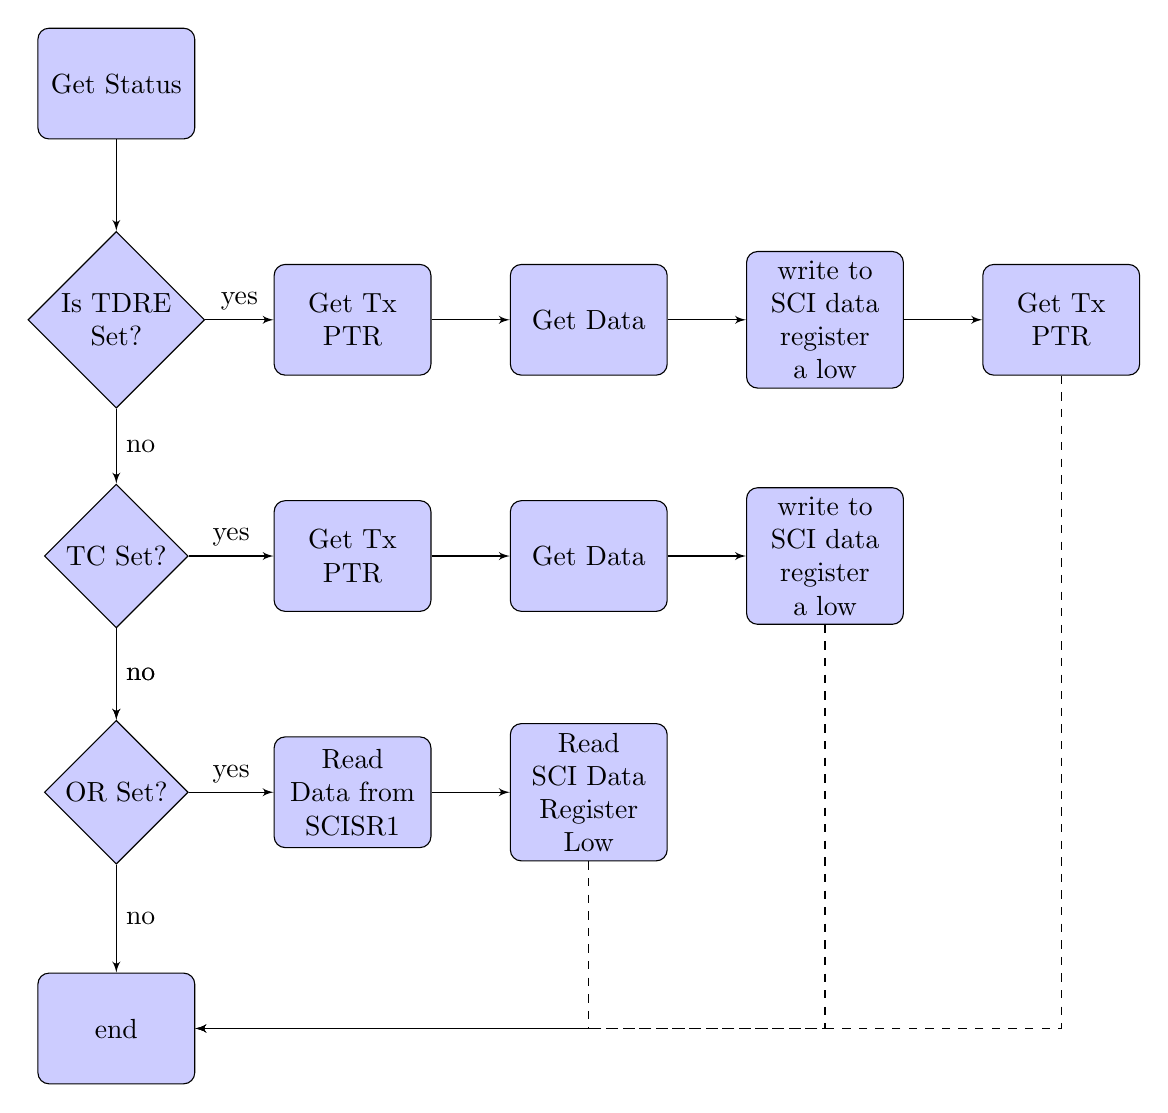
\begin{tikzpicture}[node distance = 2cm, auto]
    % Place nodes
    \node [block] (start) {Get Status};

    \node [decision, below of=start] (decide1) {Is TDRE Set?};
    \node [block, right of=decide1,node distance=3cm] (set1) {Get Tx PTR};
    \node [block, right of=set1,node distance=3cm] (set1-1) {Get Data};
    \node [block, right of=set1-1,node distance=3cm] (set1-2) {write to SCI data register a low};
    \node [block, right of=set1-2,node distance=3cm] (set1-3) {Get Tx PTR};
    
    
    \node [decision, below of=decide1] (decide2) {TC Set?};
    \node [block, right of=decide2,node distance=3cm] (set2) {Get Tx PTR};
    \node [block, right of=set2,node distance=3cm] (set2-1) {Get Data};
    \node [block, right of=set2-1,node distance=3cm] (set2-2) {write to SCI data register a low};
    
    \node [decision, below of=decide2] (decide3) {OR Set?};
    \node [block, right of=decide3,node distance=3cm] (set3) {Read Data from SCISR1};
    
    \node [block, below of=decide3,node distance=3cm] (end) {end};
    
    \node [block, right of=set3,node distance=3cm] (set3-1) {Read SCI Data Register Low};

    % Draw edges
    \path [line] (start) -- (decide1);
    \path [line] (decide1) -- node {no}(decide2);
    \path [line] (decide1) -- node {yes}(set1);
    \path [line] (decide2) -- node {no}(decide3);
    \path [line] (decide2) -- node {yes}(set2);
    \path [line] (decide3) -- node {no}(end);
    \path [line] (decide3) -- node {yes}(set3);
    
    \path [line] (set1) -- (set1-1);
    \path [line] (set1-1) -- (set1-2);
    \path [line] (set1-2) -- (set1-3);
    \path [line,dashed] (set1-3) |- (end);
    
    \path [line] (set2) -- (set2-1);
    \path [line] (set2-1) -- (set2-2);
    \path [line,dashed] (set2-2) |- (end);
    
    \path [line] (set3) -- (set3-1);
    \path [line,dashed] (set3-1) |- (end);
    
    \path [line] (decide2) -- node {no}(decide3);
\end{tikzpicture}



\end{homeworkProblem}


%----------------------------------------------------------------------------------------

\end{document}
